
\documentclass[11pt,letterpaper]{article}
\textwidth 6.5in
\textheight 9.in
\oddsidemargin 0in
\headheight 0in
\usepackage{graphicx}
\usepackage{fancybox}
\usepackage[utf8]{inputenc}
\usepackage{epsfig,graphicx}
\usepackage{multicol,pst-plot}
\usepackage{pstricks}
\usepackage{amsmath}
\usepackage{amsfonts}
\usepackage{amssymb}
% \usepackage{amsthm}
\usepackage[scr=rsfs]{mathalpha}
\usepackage{eucal}
\usepackage[left=2cm,right=2cm,top=2cm,bottom=2cm]{geometry}
\pagestyle{empty}
\DeclareMathOperator{\tr}{Tr}
\newcommand*{\op}[1]{\check{\mathbf#1}}
\newcommand{\bra}[1]{\langle #1 |}
\newcommand{\ket}[1]{| #1 \rangle}
\newcommand{\braket}[2]{\langle #1 | #2 \rangle}
\newcommand{\mean}[1]{\langle #1 \rangle}
\newcommand{\opvec}[1]{\check{\vec #1}}
\renewcommand{\sp}[1]{$${\begin{split}#1\end{split}}$$}

\usepackage{lipsum}

\usepackage{listings}
\usepackage{color}

\usepackage{theorem}
\newtheorem{thm}{Theorem}
\newtheorem{lem}[thm]{Lemma}
\newtheorem{defn}[thm]{Definition}
\newtheorem{rem}{Remark}
\def\Xint#1{\mathchoice
{\XXint\displaystyle\textstyle{#1}}%
{\XXint\textstyle\scriptstyle{#1}}%
{\XXint\scriptstyle\scriptscriptstyle{#1}}%
{\XXint\scriptscriptstyle\scriptscriptstyle{#1}}%
\!\int}
\def\XXint#1#2#3{{\setbox0=\hbox{$#1{#2#3}{\int}$ }
\vcenter{\hbox{$#2#3$ }}\kern-.6\wd0}}
\def\ddashint{\Xint=}
\def\dashint{\Xint-}

\definecolor{codegreen}{rgb}{0,0.6,0}
\definecolor{codegray}{rgb}{0.5,0.5,0.5}
\definecolor{codepurple}{rgb}{0.58,0,0.82}
\definecolor{backcolour}{rgb}{0.95,0.95,0.92}

\lstdefinestyle{mystyle}{
	backgroundcolor=\color{backcolour},   
	commentstyle=\color{codegreen},
	keywordstyle=\color{magenta},
	numberstyle=\tiny\color{codegray},
	stringstyle=\color{codepurple},
	basicstyle=\footnotesize,
	breakatwhitespace=false,         
	breaklines=true,                 
	captionpos=b,                    
	keepspaces=true,                 
	numbers=left,                    
	numbersep=5pt,                  
	showspaces=false,                
	showstringspaces=false,
	showtabs=false,                  
	tabsize=2
}

\lstset{style=mystyle}

\usepackage{tikz}
\usetikzlibrary{patterns}

\tikzset{
pattern size/.store in=\mcSize, 
pattern size = 5pt,
pattern thickness/.store in=\mcThickness, 
pattern thickness = 0.3pt,
pattern radius/.store in=\mcRadius, 
pattern radius = 1pt}
\makeatletter
\pgfutil@ifundefined{pgf@pattern@name@_dhuu1n1jk}{
\pgfdeclarepatternformonly[\mcThickness,\mcSize]{_dhuu1n1jk}
{\pgfqpoint{0pt}{-\mcThickness}}
{\pgfpoint{\mcSize}{\mcSize}}
{\pgfpoint{\mcSize}{\mcSize}}
{
\pgfsetcolor{\tikz@pattern@color}
\pgfsetlinewidth{\mcThickness}
\pgfpathmoveto{\pgfqpoint{0pt}{\mcSize}}
\pgfpathlineto{\pgfpoint{\mcSize+\mcThickness}{-\mcThickness}}
\pgfusepath{stroke}
}}
\makeatother
\tikzset{every picture/.style={line width=0.75pt}} %set default line width to 0.75pt        


\begin{document}
\pagestyle{plain}

\begin{flushleft}
Student Name: Linjie Ying\\
 Instructor:  Dr. Pengtao Sun
\end{flushleft}

\begin{flushright}\vspace{-15mm}

\includegraphics[height=1cm]{png/UNLV.png}
\end{flushright}
 
\begin{center}\vspace{0cm}
\textbf{\large Notes on Finite Element Method}\\
Assignment 1: Galerkin method on simple elliptic equations
\end{center}

 
\rule{\linewidth}{0.1mm}
%%%%%%%%%%%%%%%%%%%%%%%%%%%%%%%%%%%%%%%%%%%%%%%%%%%%%%%%%%%%%%%%%%%%%%%%

%\bigskip
%\bigskip




We intend to build a weak solution of the elliptic problem
\begin{equation}
  \label{eq:ellip}
  \begin{cases}
    -\Delta u+au&= f\textmd{ in }\Omega\\
    \alpha u+\beta \frac{\partial u}{\partial n}&=0\textmd{ on }\partial \Omega
  \end{cases}
\end{equation}
by first constructing solutions of certain finite-dimensional approximations to
a weak form of (\ref{eq:ellip})
and then passing to limits.

% \begin{thm}
%   Suppose $f\in L^2(U)$ and assume that 
% \end{thm}


\section{Weak solution}
\label{sec:weak}

\subsection{ Poisson equation with Dirichlet boundary conditions}
\label{sec:dirichlet}


First model problem:
\begin{equation}
  \label{eq:homo}
  \begin{cases}
    -\Delta u&= f\textmd{ in }\Omega\\
    u&=0\textmd{ on }\partial \Omega
  \end{cases}
\end{equation}
where $f\in L^2(\Omega)$ and $\Omega $ is open bounded subset of $\mathbb{R}^n$
with $C^1$ boundary $\partial \Omega$.
In order to define a weak solution,
we assume first that $u\in C^\infty_0$,
then multiply the equation $ -\Delta u= f$
by a smooth test function $v\in C_0^\infty$,
and integrate over $\Omega$ to find
\begin{displaymath}
  \int_\Omega \nabla u\cdot \nabla v=\int _\Omega fv,
\end{displaymath}
where we have integrated by parts on left side.
By approximation (\ref{thm:approx}) we find the same identity holds with the smooth function $v$
replaced by any $v\in H^1_0(\Omega)$,
and the resulting identity (\ref{eq:homo}) makes sense if only $u\in H^1_0(\Omega)$.
Then we get a bilinear form associated with the elliptic operator $-\Delta u$ as
\begin{equation}\label{eq:variation}
  a(u,v)=\int_\Omega \nabla u\cdot \nabla v
\end{equation}
for $u,v\in H^1_0(\Omega)$.
\begin{defn}
  We say that $u\in H_0^1(\Omega)$ is a weak solution of the boundary-value problem $(\ref{eq:homo})$
  if
  \begin{equation}\label{eq:equal}
    a(u,v)=f(v)\quad \textmd{ for all } v\in H^1_0(\Omega),
  \end{equation}
  
  where $(\ ,\ )$ denotes the inner product in $L^2(\Omega),$
  and $f(v)$ is a linear form of $f:H_0^1\rightarrow \mathbb{R}$.
\end{defn}

\paragraph{Existence and uniqueness of weak solution}
Denote semi-norm of $u\in H^m(\Omega)$ as
\begin{displaymath}
  |u|_{m,\Omega}=\left(\sum_{|\alpha|=m} \int_{\Omega}|\partial^\alpha u|^2\right)^{\frac{1}{2}}.
\end{displaymath}
We see that
\begin{displaymath}
  a(u,u)=|\nabla u|_{0,\Omega}^2
\end{displaymath}
Futhermore, $a(u,u)=0$ implies $Du = 0$ and thus $u$ is constant.
As $u=0$ on $\partial \Omega$ we have $u\equiv 0$ on $\Omega.$
Hence, $a(\cdot,\cdot )$ defines an inner product on $H^1_0$,
and then the problem (\ref{eq:equal}) has a unique solution by
Riesz Representation theorem.

Generally, use the Lax-Milgram Theorem,
which is primarily significant when it does not require symmetry of $a(\cdot, \cdot)$.
Check the two condition of $a(u,v)$,
it's obvious that
\begin{displaymath}
  |a(u,v)|\leq |\nabla u|_{0,\Omega}|\nabla v|_{0,\Omega}\leq \Vert u\Vert_{H^1_0(\Omega)}\Vert v\Vert_{H^1_0(\Omega)}.
\end{displaymath}
Use Poincare's inequality that
\begin{displaymath}
  \Vert u\Vert_{L^2(\Omega)} \leq C \Vert \nabla u\Vert_{L^2(\Omega)},
\end{displaymath}
it easily follows that
\begin{displaymath}
  \frac{1}{C}\Vert u\Vert_{H^1_0(\Omega)^2}\leq \Vert \nabla u\Vert_{L^2(\Omega)} = a(u,u).
\end{displaymath}
Futhermore the operator $f(v), v\in H_0^1(\Omega)$ is continuous by the Cauchy-Schwarz inequality,
\begin{displaymath}
  \begin{aligned}
    |f(v)|\leq \int_\Omega|f||v|\leq \Vert f\Vert_{L^2(\Omega)}\Vert v\Vert_{L^2(\Omega)}
    \leq \Vert f\Vert_{L^2(\Omega)}\Vert v\Vert_{H^1_0(\Omega)}=M\Vert v\Vert_{H^1_0(\Omega)}.
  \end{aligned}
\end{displaymath}


\paragraph{Nonhomogeneous Dirichlet condition}

A problem with prescribed, nonzero boundary values can easily be transformed into
the case of zero boundary conditions.
Suppose $\partial \Omega$ is $C^1$ and $u\in H^1(\Omega)$, $f\in L^2(\Omega)$,
let $g$ be the trace of some $H^1$ function say $w$ in the trace sense,
see theorem (\ref{thm:trace}).
Then $u$ is a weak solution of 
\begin{equation}
  \label{eq:nonhomo}
  \begin{cases}
    -\Delta u&= f\textmd{ in }\Omega\\
    u&=g\textmd{ on }\partial \Omega,
  \end{cases}
\end{equation}
which means $u=g$ on $\partial \Omega$ in the trace sense and
the identity (\ref{eq:variation}) holds for all $v\in H^1_0(\Omega)$.

In order to make $u,v$ in same space,
consider $\tilde u:= u-w$ belongs to $H^1_0(\Omega)$,
and consider $\tilde f\in H^{-1}(\Omega)$, the dual space of $H_0^1$.
Then the linear form in (\ref{eq:variation}) be
\begin{displaymath}
  (\tilde f,v)=\int_\Omega fv - a(w,v),
\end{displaymath}
and $\tilde u$ is a weak solution of the homogeneous boundary-value problem
\begin{equation}\label{pro:non-dirichlet}
  \begin{cases}
    -\Delta\tilde u&= \tilde f\textmd{ in }\Omega\\
   \tilde u&=0\textmd{ on }\partial \Omega.
  \end{cases}
\end{equation}

\begin{rem}
  \begin{displaymath}
    H^1_0(\Omega)\subset L^2(\Omega)\subset H^{-1}(\Omega)
  \end{displaymath}
\end{rem}



\section{Galerkin methods }
\label{sec:galerkin}

Consider the linear abstract variational problem:
Find $u\in V$ such that
\begin{displaymath}
  \forall v\in V, \quad a(u,v)=f(v),
\end{displaymath}
wher the space $V$ and bilinear form $a(\cdot, \cdot)$ and linear form $f$
are assumed to satisfy the assumption of the Lax-Milgram Theorem.

Then the Galerkin method for approximating the solution of such a problem
sonsists in defining similar problems in finite-dimensional subspaces of the space $V$.
\begin{defn}
  Given finite-dimensional subspace $V_h\subset V$,
  we associate the discrete problem:
  
  Find $u_h\in V_h$ such that
  \begin{displaymath}
    \forall v_h\in V_h, \quad a(u_h,v_h)=f(v_h).
  \end{displaymath}
  The unique solution $u_h$ called a \emph{discrete solution}.
\end{defn}

\textbf{Three basic aspects of conforming finite element methods}
\begin{enumerate}
\item (FEM 1) The first aspect is that a triangulation $\mathscr{T}_h$ is established over
  the set $\bar \Omega$, i.e., the set $\bar \Omega$ is subdivided into a finite number of subsets $K$,
  called finite elements, in such a way that the following properties are satisfied:
  \begin{enumerate}
  \item $\bar \Omega = \cup_{K\in \mathscr{T}_h}K.$
  \item For each $K\in \mathscr{T}_h$, the set $K$ is closed and the interior $\mathring{K}$ is nonempty.
  \item For each distinct $K_1,K_2\in \mathscr{T}_h,$ one has $\mathring{K}_1\cap \mathring{K}_2=\emptyset.$
  \item For each $K\in \mathscr{T}_h,$
    the boundary $\partial K$ is Lipschitz-continuous.
  \end{enumerate}
\item (FEM 2)
  The second basic aspect of the finite element method is that the spaces $P_K, K\in \mathscr{T}_h$,
  contain polynomials, or, at least contain functions which are "close to" polynomials.
  \begin{enumerate}
  \item it is the key to all convergence results as we shall see, and 
  \item it yields simple computations of the coefficients of the resulting linear system.
    (See below).

    Let $(w_k)_{k=1}^M$ be a basis in the space $V_h$.
    Then the solution $u_h=\sum_{k=1}^Mu_kw_k$ of problem $a(u_h,v_h)=f(v_h)$
    is such that the coefficients $u_k$
    are solutions of the linear system
    \begin{equation}
      \sum_{k=1}^Ma(w_k,w_l)u_k= f(w_l), \quad 1\leq l \leq M.
    \end{equation}
    whose matrix is always invertible,
    since the bilinear form,being assumed to be $V$-elliptic, is a fortiori $V_h$-elliptic.
  \end{enumerate}
\item (FEM 3) There exists at least one
  "canonical" basis in the space $V_h$ whose corresponding basis functions
  have supports which are as "small" as possible.
\end{enumerate}


\subsection{Finite elements}
\label{sec:finite-ele}
There are lots of different ways to construct the triangulation and spaces.
Follow the main ideas above, we give a simple example of finite elements here.




\tikzset{every picture/.style={line width=0.75pt}} %set default line width to 0.75pt        
\begin{flushright}
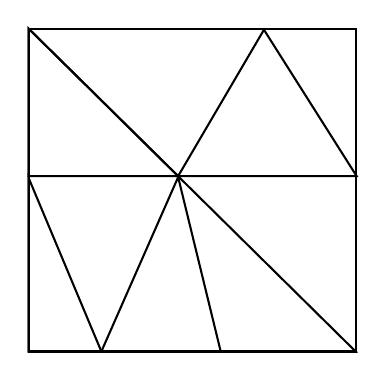
\begin{tikzpicture}[x=0.75pt,y=0.75pt,yscale=-1,xscale=1,scale=.5]
%uncomment if require: \path (0,1293); %set diagram left start at 0, and has height of 1293

%Shape: Triangle [id:dp6571094709245471] 
\draw   (100,709.97) -- (415,1020.97) -- (100,1020.97) -- cycle ;
%Shape: Rectangle [id:dp8629346324169467] 
\draw   (100,709.97) -- (415,709.97) -- (415,1020.97) -- (100,1020.97) -- cycle ;
%Shape: Right Triangle [id:dp57144005354801] 
\draw   (100,853.97) -- (170,1020.97) -- (100,1020.97) -- cycle ;
%Shape: Triangle [id:dp07020323015069474] 
\draw   (100,709.97) -- (244,851.97) -- (100,851.97) -- cycle ;
%Shape: Triangle [id:dp12561056406079496] 
\draw   (326.67,710.97) -- (244,851.97) -- (415.97,851.97) -- cycle ;
%Shape: Triangle [id:dp3321228337140698] 
\draw   (244,852.97) -- (285,1020.97) -- (170,1020.97) -- cycle ;

\end{tikzpicture}
\end{flushright}
Suppose, $\Omega\in \mathbb{R}^n$ is a polyhedral domain.
Use $n$-simplicial complex to give a triangulation ${\cal T}_h(\Omega)$.
Then a finite element in $\mathbb{R}^n$ is a triple $(K,P,\Sigma)$ where:
\begin{enumerate}
\item $K$ is a $n$-simplex of $\mathbb{R}^n$,
\item $P$ is a space of $d$-polynomials defined over the set $K$,
  with points $x_i,1\leq i\leq {n+d \choose d}$.
\item $\Sigma$ is a finite set of  nodal basis functions $\phi_i$,
  $1\leq i\leq N, N ={n+d \choose d}$, defined over the space $P$.
\end{enumerate}
Therefore, for any function $v_h|_K\in P$ we have the representation
\begin{equation}
  v_h|_K(x) = \sum _{i=1}^Nv_h(x_i)\phi_i(x).
\end{equation}
Given a finite element $(K,P,\Sigma)$ and given a function $v:K\rightarrow \mathbb{R}$
smooth,
define a project $\Pi$ 
\begin{displaymath}
 \Pi: C^\infty(K)\rightarrow P(K)\quad  \Pi v= \sum_{i=1}^N\phi_i(v)v(x_i).
\end{displaymath}

%Consider a regular family of finite elements.
\begin{defn}
  \begin{displaymath}
    \begin{aligned}
      &h_K= \textmd{ diamenter of }K,\\
      &\rho_K=\textmd{ supremum of the diameters of the spheres inscribed in K,}\\
      &h= \max_{K\in \mathscr{T}_h} h_K.
    \end{aligned}
  \end{displaymath}
\end{defn}

%\paragraph{Finite element space}

\begin{defn}
  The associated finite element space $X_h$ of problem (\ref{eq:nonhomo})
  is the subspace of the product space $\prod_{k\in \mathscr{T}_h}P_K$
  defined by
  \begin{displaymath}
    S^d_h=\left\{v_h\in H^1(\Omega):\  v|_{K}\in P_K, v_h|_{\partial \Omega}=\Pi_hg
    \right\}
  \end{displaymath}
  where $P_K$ is a space of $d$-th polynomials .
\end{defn}


Though $v_h$ is a polynomial and thus $v_h\in H^1(K)$,
it may has problem on the common boundary $\Gamma$ of
two simplex $P_1$ and $P_2$. In order to make $v_h\in H^1(\Omega)$ we need $v_h$
be continuous on the common boundaries.
Since the boundary $\Gamma\in \mathbb{R}^{n-1}$,
make enough common  points $x_i$ on $\Gamma$ we can make $v_h$ continuous on $\Gamma.$
When $n=2$ and $P$ is a space of 2-polynomials, we only need one more point,
say mid-point to make $v_h$ continuous.

\begin{center}

\tikzset{every picture/.style={line width=0.75pt}} %set default line width to 0.75pt        

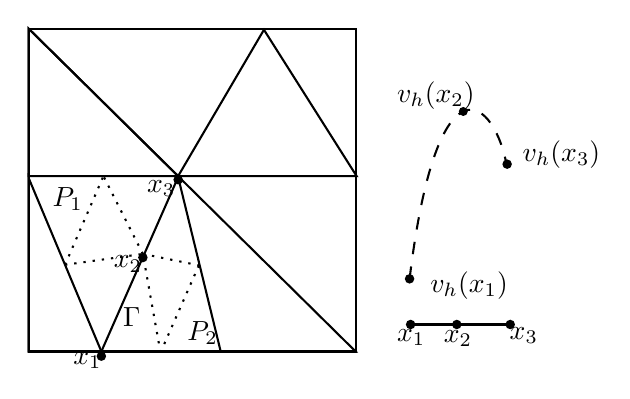
\begin{tikzpicture}[x=0.75pt,y=0.75pt,yscale=-1,xscale=1,scale=.5]
%uncomment if require: \path (0,1293); %set diagram left start at 0, and has height of 1293

%Shape: Triangle [id:dp6571094709245471] 
\draw   (100,709.97) -- (415,1020.97) -- (100,1020.97) -- cycle ;
%Shape: Rectangle [id:dp8629346324169467] 
\draw   (100,709.97) -- (415,709.97) -- (415,1020.97) -- (100,1020.97) -- cycle ;
%Shape: Right Triangle [id:dp57144005354801] 
\draw   (100,853.97) -- (170,1020.97) -- (100,1020.97) -- cycle ;
%Shape: Triangle [id:dp07020323015069474] 
\draw   (100,709.97) -- (244,851.97) -- (100,851.97) -- cycle ;
%Shape: Triangle [id:dp12561056406079496] 
\draw   (326.67,710.97) -- (244,851.97) -- (415.97,851.97) -- cycle ;
%Shape: Triangle [id:dp3321228337140698] 
\draw   (244,852.97) -- (285,1020.97) -- (170,1020.97) -- cycle ;
%Straight Lines [id:da8909801276458618] 
\draw  [dash pattern={on 0.84pt off 2.51pt}]  (135,937.47) -- (172,851.97) ;
%Straight Lines [id:da8270199793353716] 
\draw  [dash pattern={on 0.84pt off 2.51pt}]  (135,937.47) -- (210,926.97) ;
%Straight Lines [id:da24595704117595618] 
\draw  [dash pattern={on 0.84pt off 2.51pt}]  (210,926.97) -- (172,851.97) ;
%Straight Lines [id:da4085146580187684] 
\draw  [dash pattern={on 0.84pt off 2.51pt}]  (210,926.97) -- (264,937.97) ;
%Straight Lines [id:da8691705926772244] 
\draw  [dash pattern={on 0.84pt off 2.51pt}]  (227,1021.97) -- (210,926.97) ;
%Straight Lines [id:da6024758716797807] 
\draw  [dash pattern={on 0.84pt off 2.51pt}]  (227,1021.97) -- (264,937.97) ;
%Curve Lines [id:da9652227711761818] 
\draw  [dash pattern={on 4.5pt off 4.5pt}]  (467,950.97) .. controls (494,727.97) and (550,777.97) .. (561,843.97) ;
%Shape: Circle [id:dp8134257271158418] 
\draw  [color={rgb, 255:red, 0; green, 0; blue, 0 }  ,draw opacity=1 ][fill={rgb, 255:red, 0; green, 0; blue, 0 }  ,fill opacity=1 ] (240.5,855.47) .. controls (240.5,853.54) and (242.06,851.97) .. (244,851.97) .. controls (245.93,851.97) and (247.5,853.54) .. (247.5,855.47) .. controls (247.5,857.4) and (245.93,858.97) .. (244,858.97) .. controls (242.06,858.97) and (240.5,857.4) .. (240.5,855.47) -- cycle ;
%Shape: Circle [id:dp7928711929761949] 
\draw  [color={rgb, 255:red, 0; green, 0; blue, 0 }  ,draw opacity=1 ][fill={rgb, 255:red, 0; green, 0; blue, 0 }  ,fill opacity=1 ] (206.5,930.47) .. controls (206.5,928.54) and (208.07,926.97) .. (210,926.97) .. controls (211.93,926.97) and (213.5,928.54) .. (213.5,930.47) .. controls (213.5,932.4) and (211.93,933.97) .. (210,933.97) .. controls (208.07,933.97) and (206.5,932.4) .. (206.5,930.47) -- cycle ;
%Shape: Circle [id:dp5459765237158505] 
\draw  [color={rgb, 255:red, 0; green, 0; blue, 0 }  ,draw opacity=1 ][fill={rgb, 255:red, 0; green, 0; blue, 0 }  ,fill opacity=1 ] (166.5,1025.47) .. controls (166.5,1023.54) and (168.07,1021.97) .. (170,1021.97) .. controls (171.93,1021.97) and (173.5,1023.54) .. (173.5,1025.47) .. controls (173.5,1027.4) and (171.93,1028.97) .. (170,1028.97) .. controls (168.07,1028.97) and (166.5,1027.4) .. (166.5,1025.47) -- cycle ;
%Shape: Circle [id:dp8854782014634766] 
\draw  [color={rgb, 255:red, 0; green, 0; blue, 0 }  ,draw opacity=1 ][fill={rgb, 255:red, 0; green, 0; blue, 0 }  ,fill opacity=1 ] (522,789.72) .. controls (522,787.92) and (520.54,786.47) .. (518.75,786.47) .. controls (516.95,786.47) and (515.5,787.92) .. (515.5,789.72) .. controls (515.5,791.51) and (516.95,792.97) .. (518.75,792.97) .. controls (520.54,792.97) and (522,791.51) .. (522,789.72) -- cycle ;
%Shape: Circle [id:dp6273718169215265] 
\draw  [color={rgb, 255:red, 0; green, 0; blue, 0 }  ,draw opacity=1 ][fill={rgb, 255:red, 0; green, 0; blue, 0 }  ,fill opacity=1 ] (463.5,950.97) .. controls (463.5,949.04) and (465.07,947.47) .. (467,947.47) .. controls (468.93,947.47) and (470.5,949.04) .. (470.5,950.97) .. controls (470.5,952.9) and (468.93,954.47) .. (467,954.47) .. controls (465.07,954.47) and (463.5,952.9) .. (463.5,950.97) -- cycle ;
%Shape: Circle [id:dp7450362129666142] 
\draw  [color={rgb, 255:red, 0; green, 0; blue, 0 }  ,draw opacity=1 ][fill={rgb, 255:red, 0; green, 0; blue, 0 }  ,fill opacity=1 ] (557.5,840.47) .. controls (557.5,838.54) and (559.07,836.97) .. (561,836.97) .. controls (562.93,836.97) and (564.5,838.54) .. (564.5,840.47) .. controls (564.5,842.4) and (562.93,843.97) .. (561,843.97) .. controls (559.07,843.97) and (557.5,842.4) .. (557.5,840.47) -- cycle ;
%Straight Lines [id:da5472704389341718] 
\draw    (468,994.97) -- (564,994.97) ;
%Shape: Circle [id:dp9814115681023377] 
\draw  [color={rgb, 255:red, 0; green, 0; blue, 0 }  ,draw opacity=1 ][fill={rgb, 255:red, 0; green, 0; blue, 0 }  ,fill opacity=1 ] (464.5,994.97) .. controls (464.5,993.04) and (466.07,991.47) .. (468,991.47) .. controls (469.93,991.47) and (471.5,993.04) .. (471.5,994.97) .. controls (471.5,996.9) and (469.93,998.47) .. (468,998.47) .. controls (466.07,998.47) and (464.5,996.9) .. (464.5,994.97) -- cycle ;
%Shape: Circle [id:dp4051783504122395] 
\draw  [color={rgb, 255:red, 0; green, 0; blue, 0 }  ,draw opacity=1 ][fill={rgb, 255:red, 0; green, 0; blue, 0 }  ,fill opacity=1 ] (509,994.97) .. controls (509,993.04) and (510.57,991.47) .. (512.5,991.47) .. controls (514.43,991.47) and (516,993.04) .. (516,994.97) .. controls (516,996.9) and (514.43,998.47) .. (512.5,998.47) .. controls (510.57,998.47) and (509,996.9) .. (509,994.97) -- cycle ;
%Shape: Circle [id:dp59034293038065] 
\draw  [color={rgb, 255:red, 0; green, 0; blue, 0 }  ,draw opacity=1 ][fill={rgb, 255:red, 0; green, 0; blue, 0 }  ,fill opacity=1 ] (560.5,994.97) .. controls (560.5,993.04) and (562.07,991.47) .. (564,991.47) .. controls (565.93,991.47) and (567.5,993.04) .. (567.5,994.97) .. controls (567.5,996.9) and (565.93,998.47) .. (564,998.47) .. controls (562.07,998.47) and (560.5,996.9) .. (560.5,994.97) -- cycle ;

% Text Node
\draw (140,1018.97) node [anchor=north west][inner sep=0.75pt]    {$x_{1}$};
% Text Node
\draw (179,925.97) node [anchor=north west][inner sep=0.75pt]    {$x_{2}$};
% Text Node
\draw (211,852.97) node [anchor=north west][inner sep=0.75pt]    {$x_{3}$};
% Text Node
\draw (452,757.97) node [anchor=north west][inner sep=0.75pt]    {$v_{h}( x_{2})$};
% Text Node
\draw (484,940.97) node [anchor=north west][inner sep=0.75pt]    {$v_{h}( x_{1})$};
% Text Node
\draw (573,814.97) node [anchor=north west][inner sep=0.75pt]    {$v_{h}( x_{3})$};
% Text Node
\draw (452,996.97) node [anchor=north west][inner sep=0.75pt]    {$x_{1}$};
% Text Node
\draw (497,997.97) node [anchor=north west][inner sep=0.75pt]    {$x_{2}$};
% Text Node
\draw (560.5,994.97) node [anchor=north west][inner sep=0.75pt]    {$x_{3}$};
% Text Node
\draw (120,859.97) node [anchor=north west][inner sep=0.75pt]    {$P_{1}$};
% Text Node
\draw (250,988.97) node [anchor=north west][inner sep=0.75pt]    {$P_{2}$};
% Text Node
\draw (188,975.97) node [anchor=north west][inner sep=0.75pt]    {$\Gamma $};


\end{tikzpicture}
\end{center}
\section{Analysis}
\label{sec:analysis}
  The variational equations
  \begin{displaymath}
    \forall v\in V, \quad a(u,v) =f(v),
  \end{displaymath}
  satisfy the assumptions of the Lax-Milgram Theorem.

   With each finite element space $V_h$ is associated the discrete solution $u_h$
  which satisfies
  \begin{displaymath}
    \forall v_h\in V_h,\quad a(u_h,v_h)=f(v_h).
  \end{displaymath}


  \subsection{Convergence analysis}
\label{sec:convergence}
  \begin{defn}
    If $\forall f$ of the variational problem, one has
    \begin{displaymath}
      \lim_{h\rightarrow 0}\Vert u-u_h\Vert =0,
    \end{displaymath}
  Then we shall say that the associated family of discrete problems is convergent.
\end{defn}
\begin{defn}
  If a family of finite elements satisfy there exists a constant $\sigma$ such that
  $\forall h_K$, $h_K\leq \sigma \rho_K$ and $h_K$ approach zero then we call it
  \emph{a regular family of finite elements.}
\end{defn}

\subsection{Stability}
\label{sec:stability}

\paragraph{ Nonhomogeneous dirichlet  condition}

Consider the homogeneous equation problem (\ref{pro:non-dirichlet}) first.


Use Poincare's inequality for $\tilde u_h= (u-w)_h$ we have
\begin{displaymath}
  \Vert \tilde u_h\Vert_{L^2(\Omega)}\leq C\Vert D\tilde u_h\Vert_{L^2(\Omega)}
\end{displaymath}
then
\begin{displaymath}
  \Vert \tilde u_h\Vert^2_{H^1(\Omega)}=\Vert \tilde u_h\Vert_{L^2(\Omega)}^2
  +\Vert D\tilde u_h\Vert_{L^2(\Omega)}^2
  \leq  C^2\Vert D\tilde u_h\Vert_{L^2(\Omega)}^2+ \Vert D\tilde u_h\Vert_{L^2(\Omega)}^2
  =(C^2+1) \Vert D\tilde u_h\Vert_{L^2(\Omega)}^2,
\end{displaymath}
in addition, 
\begin{displaymath}
  \begin{aligned}
    \Vert D\tilde u_h\Vert_{L^2(\Omega)}^2
    &=a(\tilde u_h,\tilde u_h)
      =\tilde f(\tilde u_h)\\
    &=\int_{\Omega}f\cdot  \tilde u_h-a(w, \tilde u_h)\\
    &=\int_{\Omega}f\cdot  \tilde u_h-\int_{\Omega}Dw\cdot D\tilde u_h\\
    &\leq \Vert f\Vert_{L^2(\Omega)}\Vert \tilde u_h\Vert_{L^2(\Omega)}
      +\Vert Dw\Vert_{L^2(\Omega)}\Vert D\tilde u_h\Vert_{L^2(\Omega)}\\
    &\leq \Vert f\Vert_{L^2(\Omega)} \Vert \tilde u_h\Vert^2_{H^1(\Omega)}
      +\Vert Dw\Vert_{L^2(\Omega)} \Vert \tilde u_h\Vert^2_{H^1(\Omega)}
  \end{aligned}
\end{displaymath}
hence,
\begin{displaymath}
  \Vert \tilde u_h\Vert_{H^1(\Omega)}\leq
   \Vert f\Vert_{L^2(\Omega)} +\Vert Dw\Vert_{L^2(\Omega)}
\end{displaymath}
and the discrete solution is bounded by the given condition so the method is stable.
\subsection{Error equation}

\paragraph{Estimate of the error $\Vert u-u_h\Vert_{1}$}

Use $\Pi_h u$ denote the interpolation of $u$ in $V_h^d$,
with all $v_h|_K$ is $d$-polynomial.
Then the interpolation $\Pi_h u$ defined by $u$ has interpolation error
\begin{displaymath}
  \Vert u-\Pi _hu\Vert _{H^1(\Omega)}
  =\left (\sum_{K\in \mathscr{T}_h}\Vert u-\Pi_h u\Vert^2_{H^1(\Omega)}\right)^{1/2}.
\end{displaymath}
For all $v\in V_h\subset H_0^1(\Omega)$ we have
\begin{displaymath}
  a(\tilde u,v)=\tilde f(v),\quad a(\tilde u_h,v)= \tilde f(v)
\end{displaymath}
then the error equation is 
\begin{displaymath}
  a(\tilde u-\tilde u_h,v)=0.
\end{displaymath}
Since $\tilde u-\tilde u_h= \tilde u-\Pi_h \tilde u +\Pi_h \tilde u-\tilde u_h$, we have
\begin{displaymath}
  \Vert \tilde u-\tilde u_h\Vert_{H^1(\Omega)}
  \leq \Vert \tilde u-\Pi_h \tilde u\Vert_{H^1(\Omega)}  +\Vert\Pi_h \tilde u-\tilde u_h\Vert_{H^1(\Omega)}
\end{displaymath}
and
\begin{displaymath}
  a(\tilde u-\Pi_h \tilde u,v)+a(\Pi_h \tilde u-\tilde u_h,v)=0.
\end{displaymath}
Let $v=\Pi_h \tilde u -\tilde u_h$, then 
% $$\beta \Vert \tilde u-\Pi_h \tilde u\Vert_{H^1(\Omega)}\leq a(\tilde u-\Pi_h \tilde u,\tilde u-\Pi_h \tilde u)$$
$$\beta \Vert v\Vert_{H^1(\Omega)}^2\leq a(v,v)$$
and 
\begin{displaymath}
  a(\tilde u-\Pi_h \tilde u,v)\leq
  \alpha \Vert v\Vert _{H^1(\Omega)}
  \Vert \tilde u-\Pi_h \tilde u\Vert _{H^1(\Omega)}
\end{displaymath}
thus
\begin{displaymath}
  \Vert \Pi_h \tilde u -\tilde u_h\Vert _{H^1(\Omega)}
  \leq C\Vert \tilde u-\Pi_h \tilde u\Vert _{H^1(\Omega)}
\end{displaymath}
and
\begin{displaymath}
   \Vert \tilde u-\tilde u_h\Vert_{H^1(\Omega)}\leq (C+1)\Vert \tilde u-\Pi_h \tilde u\Vert _{H^1(\Omega)}.
 \end{displaymath}
 With all polynomials is $d$-order we have the interpolation error in semi-norm that
 $\vert \tilde u-\Pi_h \tilde u\vert _{0,\Omega}=O(h^{d+1})$
 and $\vert \tilde u-\Pi_h \tilde u\vert _{1,\Omega}=O(h^d)$,
 hence
 \begin{displaymath}
   \Vert \tilde u-\tilde u_h\Vert_{H^1(\Omega)}=O(h^d).
 \end{displaymath}
 
 
 \paragraph{Estimate of the error $\vert u-u_h\vert $}
 

 
\section{Other examples}
\label{sec:exam}


\subsection{Nonhomogeneous Neumann boundary condition}
\label{sec:neumann}
Model problem:
\begin{equation}
  \label{eq:neumann}
  \begin{cases}
    -\Delta u+u&= f\quad \textmd{ in }\Omega\\
    \frac{\partial u}{\partial n}&=g \quad \textmd{ on }\partial \Gamma
  \end{cases}
\end{equation}
with open bounded subset $\Omega\in \mathbb{R}^n$ and $f\in L^2(\Omega), g\in L^2(\partial\Omega)$.

Multiply each side with trial function $v\in C^\infty(\Omega)$ and integral in $\Omega$ we have
\begin{displaymath}
  \int_{\Omega}-\Delta u v+uv=\int_\Omega fv
\end{displaymath}
and then
\begin{displaymath}
  \int_{\Omega} \nabla u\cdot \nabla v +uv= \int_{\partial \Omega}\frac{\partial u}{\partial n}v +\int_\Omega fv
  =\int_{\partial \Omega}gv +\int_\Omega fv,
\end{displaymath}
thus we have bilinear form $H^1(\Omega)\times H^1(\Omega)\rightarrow \mathbb{R}$ that
\begin{displaymath}
  a(u,v)= \int_{\Omega} \nabla u\cdot \nabla v+uv,
\end{displaymath}
and linear form $H^1(\Omega)\rightarrow \mathbb{R}$ that 
\begin{displaymath}
  f(v)=\int_{\partial \Omega}gv +\int_\Omega fv.
\end{displaymath}

\paragraph{Existence and uniqueness}
Since
\begin{displaymath}
  |a(u,v)|\leq \int_{\Omega} |\nabla u\cdot \nabla v|+\int_\Omega |uv|
  \leq |u|_{1,\Omega}|u|_{1,\Omega}+|u|_{0,\Omega}|u|_{0,\Omega}
  \leq \Vert u\Vert_{H^1_0(\Omega)}\Vert v\Vert_{H^1_0(\Omega)},
\end{displaymath}
and
\begin{displaymath}
  a(u,u)=\int_{\Omega} |\nabla u|^2+\int_\Omega u^2=\Vert u\Vert_{H^1(\Omega)}^2,
\end{displaymath}
then $a(u,v)$ satisfies the hypotheses of the Lax-Milgram Theorem,
so that there exists a unique weak solution $u\in H^1(\Omega)$ of the variation problem
\begin{displaymath}
  a(u,v)=f(v),\quad \forall v\in H^1(\Omega).
\end{displaymath}

\paragraph{Stability}

Solve the weak form in finite-dimension to get discrete solution $u_h$ that
\begin{displaymath}
  a(u_h,v_h)=f(v_h)\quad \forall v_h\in V_h.
\end{displaymath}

\begin{displaymath}
  \begin{aligned}
    \Vert u_h\Vert_{H^1(\Omega)}^2
    &= \int_\Omega u_h\cdot u_h+\nabla u_h\cdot \nabla u_h\\
                                &=a(u_h,u_h)=f(u_h)\\
    &=\int_\Omega fu_h +\int_{\partial \Omega} gu_h\\
    &\leq \Vert g\Vert_{L^2(\partial \Omega)}\Vert u_h\Vert_{L^2(\Omega)}
      +\Vert f\Vert_{L^2(\Omega)}\Vert u_h\Vert_{L^2(\Omega)}\\
    &\leq ( \Vert g\Vert_{L^2(\partial \Omega)}+\Vert f\Vert_{L^2(\Omega)})
      \Vert u_h\Vert_{H^1(\Omega)}
  \end{aligned}
\end{displaymath}
hence
\begin{displaymath}
   \Vert u_h\Vert_{H^1(\Omega)}\leq  \Vert g\Vert_{L^2(\partial \Omega)}+\Vert f\Vert_{L^2(\Omega)}.
 \end{displaymath}

 \paragraph{Convergence and error equation}
 Since $a(u,v)$ satisfy Lax-Milgram condition,
 the error equation can be same as dirichlet boundary condition problems,
 say
 for all $v\in V_h\subset H^1(\Omega)$ we have
\begin{displaymath}
  a( u,v)= f(v),\quad a( u_h,v)=  f(v),
\end{displaymath}
then
 \begin{displaymath}
    a(u- u_h,v)=0.
 \end{displaymath}
Since $  u-  u_h=   u-\Pi_h   u +\Pi_h   u-  u_h$, we have
\begin{displaymath}
  \Vert   u-  u_h\Vert_{H^1(\Omega)}
  \leq \Vert   u-\Pi_h   u\Vert_{H^1(\Omega)}  +\Vert\Pi_h   u-  u_h\Vert_{H^1(\Omega)}
\end{displaymath}
and
\begin{displaymath}
  a(  u-\Pi_h   u,v)+a(\Pi_h   u-  u_h,v)=0.
\end{displaymath}

Let $v=\Pi_h   u -  u_h$, then 
% $$\beta \Vert   u-\Pi_h   u\Vert_{H^1(\Omega)}\leq a(  u-\Pi_h   u,  u-\Pi_h   u)$$
$$\beta \Vert v\Vert_{H^1(\Omega)}\leq a(v,v)$$
and 
\begin{displaymath}
  a(  u-\Pi_h   u,v)\leq
  \alpha \Vert v\Vert _{H^1(\Omega)}
  \Vert   u-\Pi_h   u\Vert _{H^1(\Omega)}
\end{displaymath}
thus
\begin{displaymath}
  \Vert \Pi_h   u -  u_h\Vert _{H^1(\Omega)}
  \leq C\Vert   u-\Pi_h   u\Vert _{H^1(\Omega)}
\end{displaymath}
and
\begin{displaymath}
   \Vert   u-  u_h\Vert_{H^1(\Omega)}\leq (C+1)\Vert   u-\Pi_h   u\Vert _{H^1(\Omega)}.
 \end{displaymath}
 With all polynomials is $d$-order we have the interpolation error in semi-norm that
 $\vert   u-\Pi_h   u\vert _{0,\Omega}=O(h^{d+1})$
 and $\vert   u-\Pi_h   u\vert _{1,\Omega}=O(h^d)$,
 hence
 \begin{displaymath}
   \Vert   u-  u_h\Vert_{H^1(\Omega)}=O(h^d).
 \end{displaymath}
\subsection{Robin boundary condition}
\label{sec:robin}

Model problem:
\begin{equation}
  \label{eq:neumann}
  \begin{cases}
    -\Delta u&= f\quad \textmd{ in }\Omega\\
    \frac{\partial u}{\partial n}+ \gamma u&=g \quad \textmd{ on }\partial \Gamma
  \end{cases}
\end{equation}
with open bounded subset $\Omega\in \mathbb{R}^n$ and $f\in L^2(\Omega), g\in L^2(\Omega)$, and $\gamma\neq 0$.


\paragraph{Weak solution}

To define a weak solution we multiply the equation by $v\in H^1(\Omega)$ and integrate by parts to get
\begin{displaymath}
  \begin{aligned}
    \int_\Omega -\Delta uv&= \int_\Omega \nabla u\cdot \nabla v-\int_{\partial \Omega}\frac{\partial u}{\partial n}v\\
    &= \int_\Omega \nabla u\cdot \nabla v+\int_{\partial \Omega}\gamma uv
  \end{aligned}
\end{displaymath}
then $u$ is a weak solution of
\begin{displaymath}
  \int_\Omega \nabla u\cdot \nabla v+\gamma\int_{\partial \Omega} (Tu)(Tv)=\int_\Omega fv
\end{displaymath}
where $u,v\in H^1(\Omega)$ and $T$ is trace operator, and that $Tu=u|{\partial u}$.
We define the linear form $f:H^1(\Omega)\rightarrow \mathbb{R}$ similar as previous problem that
\begin{displaymath}
  f(v)=\int_\Omega fv,
\end{displaymath}
with Cauchy-Schwarz inequality, $f$ is continuous.
We define the bilinear form $a(\cdot, \cdot):H^1(\Omega)\times H^1(\Omega)\rightarrow \mathbb{R}$ by
\begin{displaymath}
  a(u,v)= \int_\Omega \nabla u\cdot \nabla v+\gamma\int_{\partial \Omega} (Tu)(Tv)\quad \forall u,v\in H^1(\Omega)
\end{displaymath}

We prove that the bilinear form is continuous by the Cauchy-Schwarz inequality and the Trace inequality
form theorem (\ref{thm:trace}) that 
\begin{displaymath}
  \begin{aligned}
    |a(u,v)|&\leq \int_\Omega  \nabla u\cdot \nabla v+\gamma\int_{\partial \Omega} (Tu)(Tv)\\
            &\leq \Vert \nabla u\Vert_{L^2(\Omega)} \Vert \nabla v\Vert_{L^2(\Omega)}
              + \Vert Tu\Vert_{L^2(\partial\Omega)}\Vert Tv\Vert_{L^2(\partial\Omega)}\\
    &\leq \Vert \nabla u\Vert_{L^2(\Omega)} \Vert \nabla v\Vert_{L^2(\Omega)}
      + C^2\Vert u\Vert_{H^1(\Omega)}\Vert v\Vert_{H^1(\Omega)}\\
    & \leq(1+C^2) \Vert u\Vert_{H^1(\Omega)}\Vert v\Vert_{H^1(\Omega)}
  \end{aligned}
\end{displaymath}
Then we need to consider the coercivity, i.e.
we prove the statement there exists constant $\beta$ such that 
\begin{displaymath}
  \beta\Vert u\Vert_{H^1(\Omega)}\leq a(u,u).
\end{displaymath}
% Use Poincare's inequality,
% \begin{displaymath}
%   \begin{aligned}
%     \Vert u\Vert_{H^1(\Omega)}^2&
%                                   \leq \Vert u\Vert_{L^2(\Omega)}+ |u|_{1,\Omega}\\
%                                 & \leq C\Vert \nabla u\Vert_{L^2(\Omega)}+\Vert \nabla u\Vert_{L^2(\Omega)}\\
%                                 &\leq (C+1) \int_\Omega \nabla u\cdot \nabla u +(C+1)\int_{\partial \Omega} |Tu|^2\\
%     &\leq (C+1)a(u,u)
%   \end{aligned}
% \end{displaymath}

We argue by contradiction, that $a(\cdot, \cdot)$ is not coercive,
then the stated estimate false,
there would exist for each integer $k=1,\ldots,$ a function $u_k\in H^1(\Omega)$ satisfying
\begin{equation}\label{eq:1}
  \Vert u_k\Vert^2_{H^1(\Omega)}>k a(u_k,u_k).
\end{equation}
We renormalize by defining
\begin{displaymath}
  v_k=\frac{u_k}{\Vert u_k\Vert_{L^2(\Omega)}}.
\end{displaymath}
Then
\begin{displaymath}
  \Vert v_k\Vert_{L^p(\Omega)}=1,
\end{displaymath}
and the equation (\ref{eq:1}) implies that
\begin{displaymath}
  a(v_k,v_k)< \frac{1}{k}\quad (k=1,2,\ldots).
\end{displaymath}
So
\begin{equation}\label{eq:2}
  \Vert \nabla u_k\Vert_{L^2(\Omega)}^2\leq a(u,u)< \frac{1}{k},\quad
  \Vert Tv_k\Vert_{L^2(\partial \Omega)}^2< \frac{1}{k}
\end{equation}
and then $\Vert v_k\Vert^2_{H^1(\Omega)}< 1+\frac{1}{k}.$
There exist a subsequence $\{v_{k_j}\}_{j\geq 1}\subset \{v_k\}_{k\geq 1}$
and a function $v\in L^2(\Omega)$
such that
\begin{displaymath}
  v_{k_j}\rightarrow v\quad \textmd{ in }L^2(\Omega).
\end{displaymath}
It follows that
\begin{displaymath}
  \Vert v\Vert_{H^1(\Omega)}= 1.
\end{displaymath}
On the other hand,
(\ref{eq:2}) implies for $i=1,2,\ldots,n$ and  $\phi\in C^\infty_0(\Omega)$ that
\begin{displaymath}
  \int_\Omega u\phi_{x_i} \textmd{d}x=
  \lim_{k_j\rightarrow\infty}\int_{\Omega} v_{k_j}\phi_{x_i}\textmd{d}x
  =- \lim_{k_j\rightarrow\infty}\int_{\Omega} v_{k_j,x_i}\phi\textmd{d}x=0
\end{displaymath}
Consequently $v\in H^1(\Omega)$ with $\nabla v=0$.
Thus $v$ is constant on each component of $\Omega$.
But
\begin{displaymath}
  \Vert Tv\Vert_{L^2(\partial \Omega)}
  \leq \Vert T(v-v_k)\Vert_{L^2(\partial \Omega)}+\Vert Tv_k\Vert_{L^2(\partial \Omega)}
  \leq \Vert T\Vert \Vert v-v_k\Vert_{L^2(\partial \Omega)}+\sqrt{\frac{1}{k}}
  \rightarrow 0\quad \textmd{ as }k\rightarrow \infty.
\end{displaymath}
which means $v\equiv 0$ on $\partial \Omega$ and hence $v\equiv 0$ on $U$.
This contradicts to $\Vert v\Vert_{H^1}=1$.
Therefore $a(\cdot,\cdot)$ is coercive.

The
Lax-Milgram theorem then gives a unique weak solution.
\paragraph{Stability}
Use the coercive of $a(\cdot, \cdot)$ we have
\begin{displaymath}
  \beta\Vert u_h\Vert_{H^1(\Omega)}^2
  \leq a(u_h,u_h)= f(u_h)
  \leq \Vert f\Vert_{L^2(\Omega)}\Vert u_h\Vert_{L^2(\Omega)}
  \leq \Vert f\Vert_{L^2(\Omega)}\Vert u_h\Vert_{H^1(\Omega)}
\end{displaymath}
and then
\begin{displaymath}
  \Vert u_h\Vert_{H^1(\Omega)}\leq C \Vert f\Vert_{L^2(\Omega)}.
\end{displaymath}

\paragraph{Error equation}
Similar as previous question since $a(\cdot, \cdot)$ and $f$ satisfies condition of Lax-Milgram Theorem.
\section{Sobolev spaces}
\label{sec:sobolev}



\begin{thm}[Global approximation by funcitons smooth up to the boundary]
  \label{thm:approx}
  Assume $U$ is bounded and $\partial U$ is $C^1$.
  Suppose $u\in W^{k,p}(U)$ for some $1\leq p <\infty$.
  Then there exist functions $u_m\in C^\infty(\bar U)$ such that
  \begin{displaymath}
    u_m\rightarrow u\quad \textmd{ in }W^{k,p}(U).
  \end{displaymath}
\end{thm}


\begin{thm}[Trace Theorem]
  \label{thm:trace}
  Assume $U$ is bounded and $\partial U$ is bounded and $\partial U$ is $C^1$.
  Then there exists a bounded linear operator
  \begin{displaymath}
    T: W^{1,p}(U)\rightarrow L^p( \partial U)
  \end{displaymath}
  such that
  \begin{enumerate}
  \item $Tu=u|_{\partial U}$ if $u\in W^{1,p}(U)\cap C(\bar U)$
  \item
   $
      \Vert Tu\Vert _{L^p(\partial U)}\leq C\Vert u\Vert_{W^{1,p}(U)}$
 
  \end{enumerate}
  for each $u\in W^{1,p}(U)$, with the constant $C$ depending only on $p$ and $U$.
\end{thm}

\begin{thm}[Lax-Milgram Theorem]
  \label{eq:lax}
  Let $V$ be a Hilbert space, let $a(\cdot,\cdot):V\times V\rightarrow \mathbb{R}$
  be a continuous $V$-elliptic bilinear form, which means there exist constant $\alpha,\beta>0$
  such that
  \begin{displaymath}
    |a(u,v)|\leq \alpha \Vert u\Vert \Vert v\Vert,\quad (u,v\in V)
  \end{displaymath}
  and satisfy the coercivity condition
  \begin{displaymath}
    \beta\Vert u\Vert^2\leq a(u,u)\quad (u\in V).
  \end{displaymath}
  and let $f:V\rightarrow \mathbb{R}$ be a continuous linear form.

  Then the abstract variational problem: Find an element $u$ such that
  \begin{equation}
    \label{eq:l}
    u\in V\quad \textmd{ and }\quad \forall v\in V,\quad  a(u,v)=f(v)
  \end{equation}
  has one and only one solution.
\end{thm}


\begin{thm}(C\'{e}a's lemma)
  There exists a constant $C$ independent upon the subspace $V_h$ such that
  \begin{displaymath}
    \Vert u-u_h\Vert \leq C\inf_{v_h\in V_h}\Vert u-v_h\Vert.
  \end{displaymath}
\end{thm}

\end{document}






